% The 22 primes at most 80. A charcoal bar marks a prime \equiv 1 (mod 4): nine primes.
% A coral bar marks a prime \equiv 3 (mod 4): twelve primes. The prime 2 has no bar.
% Order: 2, 3, 5, 7, 11, 13, 17, 19, 23, 29, 31 and 37, 41, 43, 47, 53, 59, 61, 67, 71, 73, 79.
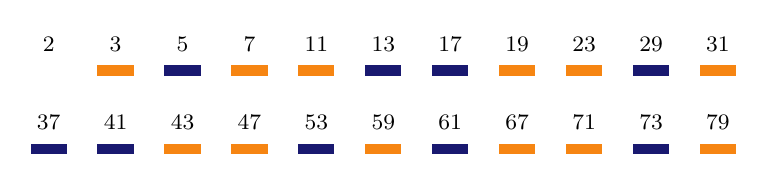
\begin{tikzpicture}[every node/.style={font=\footnotesize}]
  \node at (0.40,1.35) {$2$};
  \node at (1.25,1.35) {$3$};
  \fill[BurntOrange] (1.02,0.95) rectangle (1.48,1.08);
  \node at (2.10,1.35) {$5$};
  \fill[MidnightBlue] (1.87,0.95) rectangle (2.33,1.08);
  \node at (2.95,1.35) {$7$};
  \fill[BurntOrange] (2.72,0.95) rectangle (3.18,1.08);
  \node at (3.80,1.35) {$11$};
  \fill[BurntOrange] (3.57,0.95) rectangle (4.03,1.08);
  \node at (4.65,1.35) {$13$};
  \fill[MidnightBlue] (4.42,0.95) rectangle (4.88,1.08);
  \node at (5.50,1.35) {$17$};
  \fill[MidnightBlue] (5.27,0.95) rectangle (5.73,1.08);
  \node at (6.35,1.35) {$19$};
  \fill[BurntOrange] (6.12,0.95) rectangle (6.58,1.08);
  \node at (7.20,1.35) {$23$};
  \fill[BurntOrange] (6.97,0.95) rectangle (7.43,1.08);
  \node at (8.05,1.35) {$29$};
  \fill[MidnightBlue] (7.82,0.95) rectangle (8.28,1.08);
  \node at (8.90,1.35) {$31$};
  \fill[BurntOrange] (8.67,0.95) rectangle (9.13,1.08);
  \node at (0.40,0.35) {$37$};
  \fill[MidnightBlue] (0.17,-0.05) rectangle (0.63,0.08);
  \node at (1.25,0.35) {$41$};
  \fill[MidnightBlue] (1.02,-0.05) rectangle (1.48,0.08);
  \node at (2.10,0.35) {$43$};
  \fill[BurntOrange] (1.87,-0.05) rectangle (2.33,0.08);
  \node at (2.95,0.35) {$47$};
  \fill[BurntOrange] (2.72,-0.05) rectangle (3.18,0.08);
  \node at (3.80,0.35) {$53$};
  \fill[MidnightBlue] (3.57,-0.05) rectangle (4.03,0.08);
  \node at (4.65,0.35) {$59$};
  \fill[BurntOrange] (4.42,-0.05) rectangle (4.88,0.08);
  \node at (5.50,0.35) {$61$};
  \fill[MidnightBlue] (5.27,-0.05) rectangle (5.73,0.08);
  \node at (6.35,0.35) {$67$};
  \fill[BurntOrange] (6.12,-0.05) rectangle (6.58,0.08);
  \node at (7.20,0.35) {$71$};
  \fill[BurntOrange] (6.97,-0.05) rectangle (7.43,0.08);
  \node at (8.05,0.35) {$73$};
  \fill[MidnightBlue] (7.82,-0.05) rectangle (8.28,0.08);
  \node at (8.90,0.35) {$79$};
  \fill[BurntOrange] (8.67,-0.05) rectangle (9.13,0.08);
\end{tikzpicture}
